
\chapter{Experiments and Results}
\label{chapter:experiments-and-results}
This chapter extends upon the information extraction task using convolutional neural networks as described in the previous sections. We primarily aim to extract the relational information from preprocessed biomedical texts in the form of tuples of {\it <stage, ethnicity>} and {\it <stage, sample size>} and therefore, reach the final entries for the GWAS catalog. The extraction of these semantic data is executed as two separate tasks with Task 1 as identification of pairs of stage and ethnicity groups and Task 2 being the identification of tuples of stage and sample size. These tasks are further described in Figure \ref{figure:task-example} with the help of an example. This chapter focuses on the experiments undertaken for these tasks and the comparison of the results for the same. We begin with a description of our experiment strategy including the information on the dataset used, training and testing process and hyper-parameters settings for the neural network. Following this, we report our experiments for the two tasks using different neural networks (as described in the previous chapter) and their corresponding results.

\begin{figure}[ht]
    \centering
    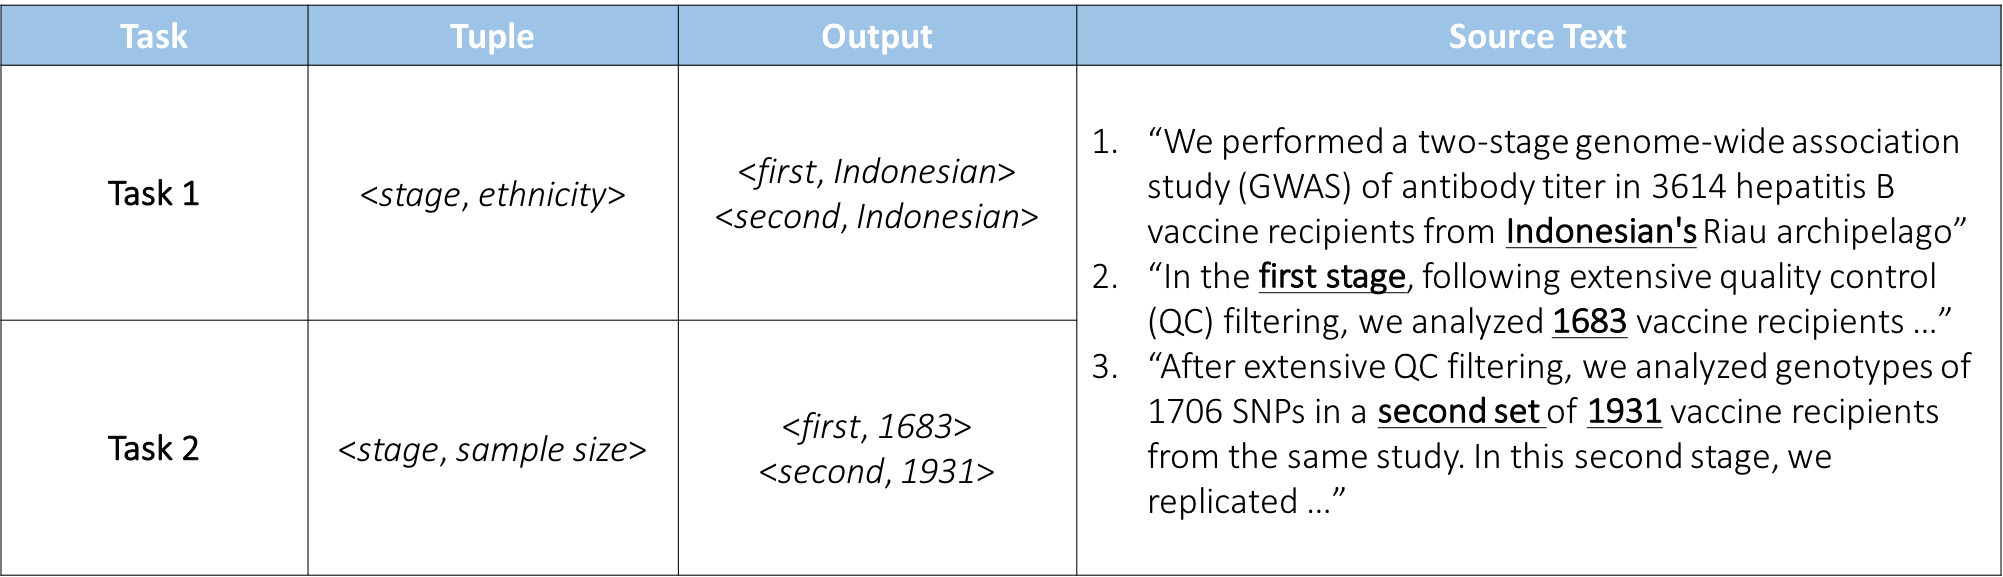
\includegraphics[width=0.85\linewidth]{Images/Task-Example.png}
    \caption{An illustration of the two relation extraction tasks along with example tuples extracted from the source text.}
    \label{figure:task-example}
\end{figure}

\section{Experiments Metrics}
\label{section:experiment-metrics}
For each task described previously, we follow a pipeline structure where the computation begins with an input document and finally produces the relational tuple as required for the operation. The PDF file used as input goes through a series of pre-processing steps like PDF-to-XML conversion, XML-to-Text transcription, entity tagging and vector creation as described in Chapter \ref{chapter:data-preprocessing}. These tagged entity candidates (in the form of vectors) are used to train the neural network model with truth values extracted from the existing entries in GWAS catalog. Therefore, we need to create the training data using biomedical literature which have been already curated and added to the catalog. The two relation extraction tasks follow a shared data preprocessing pipeline but have separate neural networks as the underlying structure in the text for these tasks could be very different from each other. These neural networks are similar in the overall architecture but are trained and run independently to avoid the overlap of one task with another.

As already discussed, our dataset for the experiments is created using the articles which are already curated and have been entered into the catalog of GWAS. This data is available freely in form of a spreadsheet and can be obtained from the NHGRI page\footnote{\url{https://www.genome.gov/26525384/}}. We selected the articles that satisfied the following criteria:

\begin{itemize}
    \item \emph{Curated data available}:
    2,185 PubMed articles were curated with the data available to start with.
    
    \item \emph{NXMLs or PDFs available}:
    We used NXML version of the articles if they are available through PubMed Central. These versions have high-quality text and we can ignore the PDF-to-XML conversion step while using these files. Otherwise, we transcribed PDF versions of the remaining articles to text. This excludes 324 articles and leaves 1,861 articles.
    
    \item \emph{No missing values or ``NR''}:
    The characteristics of the samples are available for whichever stage is mentioned in the article, and the curated data contains no blank entries. Also, excluded are those articles for which curators were unable to find a conclusive ethnicity group for the sample and the entries state ``NR'' (``not reported''). This step leaves us with 1,674 articles.
    
    \item \emph{Ethnicty metions in Text}:
    Terms that corresponds to ethnic groups must be available in text (and not inferred from affiliations of authors, for example), leaving 1,130 articles.
    
    \item \emph{Sample Size mentions in Text}:
    The sample size is present in the text as a number and not inferred from some other description. Also, it is important for the value of sample size to be present in the textual context. 
    
    \item \emph{Does not contain Errors}:
    The articles were excluded for which the curated data was found to contain errors in their entries.
\end{itemize}

The final dataset for the Task 1 consists of 1,311 articles, comprising of 2,357 {\it <stage, ethnicity>} tuples. Similarly, for Task 2 only 409 articles comprising of 657 {\it <stage, sample size>} tuples were used for the training of neural network. Along with these positive examples, there were multiple negative examples that were automatically created by the imperfections while tagging the entity mentions in the input text. Out of these, an intersection of 92 articles and 300 tuples articles comprised of the dataset for evaluation of the trained networks.

Before the training process, these dataset articles along with the tagged entities need to be converted to a form that is understood by the neural networks. As discussed in previous sections, the pre-trained word embeddings\footnote{\url{http://bio.nlplab.org/}} \cite{pyysalo2013distributional} were created using the \emph{word2vec} tool on a huge corpus of biomedical literature and have a dimensionality of 8. Also, the positional embeddings of size 2 were used to represent each candidate mentions and its location with respect to other tokens in the text. We entered a set of 30 words along with the marked entities to the network for the processing. The input to the system was, therefore, a matrix of size $12 \times 30$ and was treated as an ``image'' for the convolution process.

The dataset for the two tasks is used to train their corresponding neural networks using the Stochastic Gradient Descent (SGD) method. For each of the tasks, five-fold article based cross-validation (5-fold CV) is performed during the training phase. The articles in the dataset are shuffled randomly, and each fold utilizes all the tuples belonging to $80\%$ of the articles in the dataset as training data, and the tuples in the remaining $20\%$ of the articles as validation data. The gradients for each neuron were computed using the back-propagation of errors through multiple layers and the filter weights were adjusted in each iteration accordingly. Each training iteration was done with shuffled mini-batches of size 50 and the AdaDelta update rule \cite{zeiler2012adadelta} with a dropout rate of 0.5. For all the experimental runs, we used $tanh$ for the non-linear activation and 150 filters for each window size in the model. 

To assess the performance of our system, we compare the results on the evaluation dataset with the previous work in the same domain \cite{kashyapthesis}. The key idea of this work was to use a {\it cost-sensitive} learning algorithm to learn from the training examples weighted by an estimated reliability of each example. This approach involved extracting a huge number of token-based, context-based and other features from the text which were entered into a committee of weak classifiers. These classifiers, varying from simple binary classifiers to rule-based-classifiers, were used to estimate the cost to be assigned to each training instance. These costs were then used to train a L$_{2}$-regularized, linear support vector machine (SVM) to classify each example as a positive or negative instance. Overall, it can be surmised that our baseline model was based on extensive feature modeling and engineering using different natural language modules, and an SVM classifier for the mentioned information extraction task.

The result for each task is then collected to obtain the corresponding tuples for all the articles in the evaluation dataset. These results are compared against the curated data and F1 score calculated in the standard way:

\begin{itemize}[noitemsep]
    \item If a tuple in the result for a specific article is present in the curated data for that article, it is considered a true positive (TP); otherwise, it is considered a false positive (FP)
    
    \item If a tuple in the curated data for a specific article does not have a counterpart in the extracted results, it is considered a false negative (FN). 
\end{itemize}

Using this we calculate the precision, recall and F-1 score for each task and compare it against the baseline method for the same dataset. These results are discussed in further details for different neural networks in the upcoming sections.

\section{Default Parameters}
\label{section:default-parameters}
We measure the effectiveness of our architecture for the task of relation extraction by running experiments for each task as described in the previous sections. We start with designing our neural network model with the default parameters as listed in Table \ref{table:basic-configuration} and evaluate them for our tasks. The main idea is to understand how well our primary system would perform in comparison to the previous existing models. The outcome from these runs guides us to add extensions and change settings in the model to improve the performance further. 

We train our models for the two tasks using their respective datasets using the stochastic gradient descent methods as mentioned in the previous section. After this, we evaluate these models using the test dataset to extract pairs of {\it <stage, ethnicity>} for Task 1 and {\it <stage, sample size>} for Task 2 as required. These results are summarized in Table \ref{table:basic-results} with the corresponding baselines for each of these tasks. It is evident from the table that we are not performing significantly better in comparison to the existing systems, especially for Task 1 where the F-1 scores are exactly same as before.

However, these results show that our neural network model successfully captures the underlying semantic and syntactic structure of the text and can be used for the relation extraction task to perform equally good as the existing models. Also, as current results are based on a model with default parameters, we believe that extending our framework would lead to better results for our tasks. Having established a baseline performance for the convolutional neural networks for these jobs, we consider the effect of different architecture decisions and hyperparameters settings in next sections.

\begin{table}[ht]
    \centering
    \caption{Performance of our model with basic configuration (Neural Network Model) as listed in Table \ref{table:basic-configuration} for each of the two tasks and its comparison against the previous work (Baseline Model).}
    \begin{tabular}{c  c  c  c}
         \toprule
         \textbf{Task Description}  &   \textbf{Precision}      &   \textbf{Recall}            &   \textbf{F-1 Score}      \\
         \midrule
         \multicolumn{4}{c}{Task 1}                             \\
         \hline
         \\[-1em]
         
         Baseline Model             &   0.74                    &             0.77                       &   0.75                    \\
         
         Neural Network Model       &   0.73                    &             0.79                       &   0.75                    \\
         
         \midrule
         \multicolumn{4}{c}{Task 2}                            \\
         \hline
         \\[-1em]
         
         Baseline Model             &   0.56                    &             0.74                       &   0.64                    \\
         
         Neural Network Model       &   0.68                    &             0.70                       &   0.69                    \\
         
         \bottomrule
    \end{tabular}
    \label{table:basic-results}
\end{table}

\section{Filter Sizes Extension}
\label{section:filter-sizes-extension}
Although the results with basic parameters are quite good and comparable to the existing system, they can be further enhanced by extending the current neural network model. One way to achieve this is to change the filter region sizes and study its effect on the overall performance of the model. As already discussed in previous sections, this would modify the quality of our model as different filter sizes would result in different windows of text being captured in the convolutional layer, from which subsequent features are extracted. We consider region sizes of 1, 3, 4, 5, 7, 8 and 10 while keeping the other parameters fixed and record the results of our experiments for both tasks. These results are reported in Table \ref{table:task1-filter-size-results} for the first task of extraction of {\it <stage, ethnicity>} tuples and Table \ref{table:task2-filter-size-results} for second task of extractions of pairs of {\it <stage, sample size>}. 

From these results, one can see that each task has its optimal filter region size. The table also suggests that a reasonable range for relation extraction tasks might be from 5 to 7 for our domain of biomedical literature. The filter size extension is not only able to achieve a much higher degree of recall, but this improvement is also accompanied by an increase in the overall precision as well. We can use these optimal filter region sizes to improve further the performance of our model using another extension as described in next section. 
\begin{table}[ht]
    \centering
    \caption{Performance of our convolutional neural network with different filter region sizes for Task 1}
    \begin{tabular}{c  c  c  c}
         \toprule
         \textbf{Filer Size}        &   \textbf{Precision}      &   \textbf{Recall}            &   \textbf{F-1 Score}      \\
         \midrule
         \\[-1em]
         
         Baseline                   &   0.74                    &            0.77                       &   0.75                    \\

         1                          &   0.52                    &             0.66                       &   0.58                    \\

         3                          &   0.71                    &             0.77                       &   0.73                    \\

         4                          &   0.73                    &             0.79                       &   0.75                    \\
         
         5                          &   0.74                    &             0.80                       &   0.76                    \\
         
         \textbf{7}                 &   \textbf{0.77}           &             \textbf{0.82}              &   \textbf{0.79}           \\
         
         8                          &   0.73                    &             0.79                       &   0.75                    \\
         
         10                         &   0.69                    &             0.73                       &   0.71                    \\
         
         \bottomrule
    \end{tabular}
    \label{table:task1-filter-size-results}
    \vspace{0.1in}
\end{table}

\begin{table}[ht]
    \centering
    \caption{Performance of our convolutional neural network with different filter region sizes for Task 2}
    \begin{tabular}{c  c  c  c}
         \toprule
         \textbf{Filer Size}        &   \textbf{Precision}      &   \textbf{Recall}            &   \textbf{F-1 Score}      \\
         \midrule
         \\[-1em]
         
         Baseline                   &   0.55                    &            0.74                       &   0.63                    \\

         1                          &   0.42                    &             0.57                       &   0.48                    \\

         3                          &   0.55                    &             0.70                       &   0.61                    \\

         4                          &   0.58                    &             0.73                       &   0.65                    \\
         
         \textbf{5}                 &   \textbf{0.62}           &             \textbf{0.77}              &   \textbf{0.69}           \\
         
         7                          &   0.60                     &            0.79                       &   0.68                    \\
         
         8                          &   0.57                    &             0.77                       &   0.66                    \\
         
         10                         &   0.54                    &             0.72                       &   0.62                    \\
         
         \bottomrule
    \end{tabular}
    \label{table:task2-filter-size-results}
\end{table}

\section{Filter Combinations Extension}
\label{section:filter-combinations-extension}
The performance of our neural network model is highly improved upon changing the filter region sizes in comparison to default parameters or baseline models. This development motivated us to combine multiple filter sizes into a single architecture to capture the maximum possible combination of features in a single unified neural network model. As such, we explored the effect of combining different filter region sizes, while keeping all the other parameters fixed as before. The number of filter sizes was also increased such that each of the region sizes had 150 filters as before. The result of the experiments conducted with these multiple filter sizes are recorded in Table \ref{table:task1-multiple-filter-results} and \ref{table:task2-multiple-filter-results} for Task 1 and Task 2 respectively. 

As can be directly inferred from the two tables, the optimal combination of filters is different from the two tasks which are similar to the observation from last experiments. Also, for each of the tasks, it can be noted that the combination of various filters with region sizes akin to the optimal single region size improves the performance drastically in comparison to adding region sizes far from the optimal range. The best results we are able to achieve for our neural network model are an F-1 score of 0.85 for extraction of {\it <stage, ethnicity>} tuples and an F-1 score of 0.74 to extract pairs of {\it <stage, sample size>}.

\begin{table}[ht]
    \centering
    \caption{Performance of our convolutional neural network with multiple filter region size combinations for Task 1}
    \begin{tabular}{c  c  c  c}
         \toprule
         \textbf{Filer Size}        &   \textbf{Precision}      &   \textbf{Recall}            &   \textbf{F-1 Score}      \\
         \midrule
         \\[-1em]
         
         Baseline                   &   0.74                    &            0.77                       &   0.75                    \\

         7                          &   0.77                    &             0.82                       &   0.79                    \\
         
         [2, 3, 4]                  &   0.80                    &             0.84                       &   0.82                    \\

         [3, 4, 5]                  &   0.83                    &             0.85                       &   0.84                    \\

         \textbf{[3, 5, 8]}         &   \textbf{0.84}           &             \textbf{0.87}              &   \textbf{0.85}           \\
         
         [5, 7, 8]                  &   0.83                     &            0.84                       &   0.83                    \\
         
         \bottomrule
    \end{tabular}
    \label{table:task1-multiple-filter-results}
    \vspace{0.2in}
\end{table}

\begin{table}[ht]
    \centering
    \caption{Performance of our convolutional neural network with multiple filter region size combinations for Task 2}
    \begin{tabular}{c  c  c  c}
         \toprule
         \textbf{Filer Size}        &   \textbf{Precision}      &   \textbf{Recall}            &   \textbf{F-1 Score}      \\
         \midrule
         \\[-1em]
         
         Baseline                   &   0.55                    &            0.74                       &   0.63                    \\

         5                          &   0.62                    &             0.77                       &   0.69                    \\
         
         [2, 3, 4]                  &   0.66                    &             0.78                       &   0.71                    \\

         \textbf{[3, 4, 5]}         &   \textbf{0.69}           &             \textbf{0.81}              &   \textbf{0.74}           \\

         [3, 5, 8]                  &   0.68                    &             0.79                       &   0.73                    \\
         
         [5, 7, 8]                  &   0.65                     &            0.76                       &   0.70                    \\
         
         \bottomrule
    \end{tabular}
    \label{table:task2-multiple-filter-results}
\end{table}

Material from chapter \ref{chapter:experiments-and-results} in part is currently being prepared for submission for the publication of material. The thesis author was the primary investigator and author of this material. 
